%==================================================================
\frame{\frametitle{Ecological networks}
  
  Networks = natural way do depict the ({\sl direct}) interactions between entities, including living species \refer{PSK16}
  
  \bigskip
  \begin{tabular}{ll}
   \paragraph{Trophic network.} & \paragraph{Microbial network.} \refer{FaR12} \\
   \begin{tabular}{p{.45\textwidth}}
    $$
    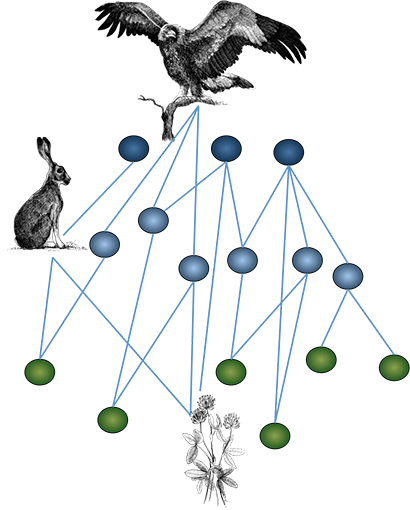
\includegraphics[width=.3\textwidth]{\figeco/ecological-networks-and-community-ecology50}
    $$
   \end{tabular}
   &
   \begin{tabular}{p{.45\textwidth}}
    $$
    \includegraphics[width=.45\textwidth]{\figeco/FaR12-Nature-Fig3a}
    $$
   \end{tabular}
  \end{tabular}
}

%==================================================================
\frame{\frametitle{Two different situations}

  \paragraph{Interactions are not-observed.} 
  \begin{itemize}
   \item Species abundance or presence/absence data (co-occurrence 'networks')
   \item Deep sequencing, metagenomics
  \end{itemize}
  \ra Reconstruct the 'interaction' network \ra \emphase{Lecture 1}

  \bigskip \bigskip 
  \paragraph{Interactions are observed.} 
  \begin{itemize}
   \item Interaction networks, contact networks
   \item Trophic networks, plant-pollinators networks
  \end{itemize}
  \ra Understand the organization/functioning  of the network \ra \emphase{Lecture 2}


}

%==================================================================
\frame{\frametitle{Network reconstruction}

  \paragraph{Generic problem:} $n$ sites, $p$ species, $d$ covariates
  
\pause \hspace{-0.06\textwidth}
\begin{tabular}{c|c|l}
  \onslide+<2->{\paragraph{Abundances:} $Y = n \times p$}
  & 
  \onslide+<3->{\paragraph{Covariates:} $X = n \times d$}
  & 
  \onslide+<4>{\paragraph{Network:} $G = p \times p$ }
  \\
  \hspace{-.02\textwidth} 
  \begin{tabular}{p{.28\textwidth}}
    \onslide+<2->{\begin{tabular}{rrr}
      {\sl Hi.pl} & {\sl An.lu} & {\sl Me.ae} 
      %\footnote{{\sl Hi.pl}: Long rough dab, {\sl An.lu}: Atlantic wolffish, {\sl Me.ae}: Haddock} 
      \\ 
%       Dab & Wolffish & Haddock \\ 
      \hline
      31  &   0  & 108 \\
       4  &   0  & 110 \\
      27  &   0  & 788 \\
      13  &   0  & 295 \\
      23  &   0  &  13 \\
      20  &   0  &  97 \\
      \vdots & \vdots & \vdots 
    \end{tabular}} 
  \end{tabular}
  & 
  \begin{tabular}{p{.3\textwidth}}
    \onslide+<3->{\begin{tabular}{rrr}
      Lat. & Long. & Depth \\ \hline
      71.10 & 22.43 & 349 \\
      71.32 & 23.68 & 382 \\
      71.60 & 24.90 & 294 \\
      71.27 & 25.88 & 304 \\
      71.52 & 28.12 & 384 \\
      71.48 & 29.10 & 344 \\
      \vdots & \vdots & \vdots 
    \end{tabular}} 
  \end{tabular}
  & 
  \hspace{-.02\textwidth} \pause
  \begin{tabular}{p{.3\textwidth}}
    \onslide+<4>{\hspace{-.1\textwidth} 
      \begin{tabular}{c}
        \includegraphics[width=.35\textwidth]{\figCMR/network_BarentsFish_Gfull_full60edges}
      \end{tabular}}
  \end{tabular}
\end{tabular}
  
\begin{itemize}
\item sites could be dates, positions along a gradient
\item 'abundances' could be presence/absence, read counts, etc..
\end{itemize}

\bigskip 
\onslide+<4>{\paragraph{Goal:} infer $G$ based on $X$ and $Y$.}
}

%==================================================================
\frame{\frametitle{Not an easy task}

  \paragraph{A huge search space:}
  $$
  \includegraphics[trim=50 50 0 75, height=.5\textheight, clip]{\fignet/NbGraphs}
  $$
  Number of \textcolor{darkgreen}{undirected graphs} ($2^{p(p-1)/2}$), \textcolor{red}{directed acyclic graphs} (no close form), \textcolor{blue}{spanning trees} ($p^{p-2}$)
}
